\documentclass[handout]{beamer}
\usepackage{booktabs}
\usepackage{langsci-optional}
\usepackage{fontspec} 
% \usepackage{lsp-makros}
\useoutertheme{lsp}

\usepackage{lsptitle}

\def\two@digits#1{\ifnum#1<10 0\fi\number#1}
\def\mytoday{\two@digits{\number\day}.\two@digits{\number\month}.\number\year}


\usepackage{xspace,multicol}
\newcommand{\latex}{\LaTeX\xspace}
\usepackage{tikz}


\newcounter{lastpagemainpart}
\footnotesep0pt
\renewcommand{\footnoterule}{}
\usefootnotetemplate{
  \noindent
  \insertfootnotemark\insertfootnotetext}

\let\beamerfn=\footnote
\renewcommand{\footnote}[1]{%
\let\oldfnsize=\footnotesize%
\let\footnotesize=\tiny%
\beamerfn<\thebeamerpauses$\to${#1}%
\let\footnotesize=\oldfnsize}


\date{\today}

\usepackage{eurosym}  
 
\renewcommand{\centerline}[1]{\hfill#1\hfill\hfill\mbox{}}


\title{Phonological cover-up:\\ \normalsize Contact-induced undoing of sound changes in Sri Lanka Malay}
\institute{Language Science Press}
\author[Nordhoff]{Sebastian Nordhoff}
\date{2022-08-02, ICHL 25, University of Oxford}


\usepackage[
	natbib=true,
	style=langsci-unified,
	%refsection=chapter,
	maxbibnames=99,
	uniquename=false,
	mincrossrefs=99,
	maxcitenames=2,
	isbn=false,
	autolang=hyphen,
]{biblatex}


\begin{document}
\lspbeamertitle


raasa vs. rasa Sinhala
kuuda vs kudhai Tamil
moraic restriction save the day kudda or rassa would not match Sinh/Tam



\section{Language change}
\frame{
\frametitle{A typology of language change}
 \begin{itemize}
    \item   no change
    \item   internal change
    \item   contact-induced change
    \item   contact-induced non-change
    \item   contact-induced reversal
 \end{itemize}
}

\frame{
\frametitle{No change}
\vspace*{1cm}
  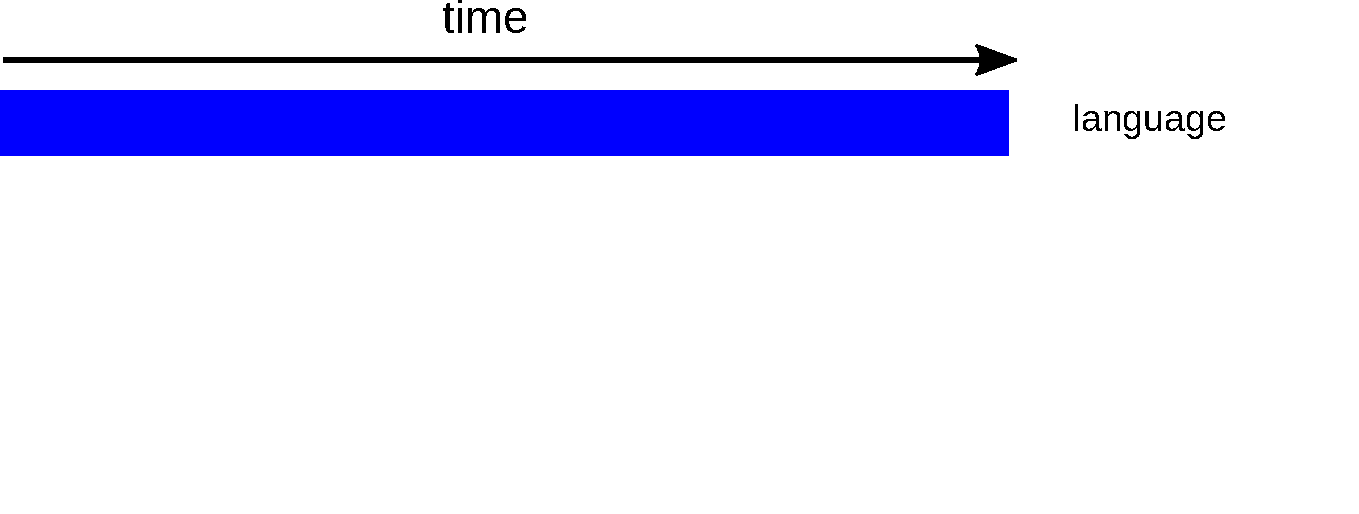
\includegraphics[width=\textwidth]{nochange.pdf}\vfill ~
}


\frame{
\vspace*{1cm}
\frametitle{Internal change}
  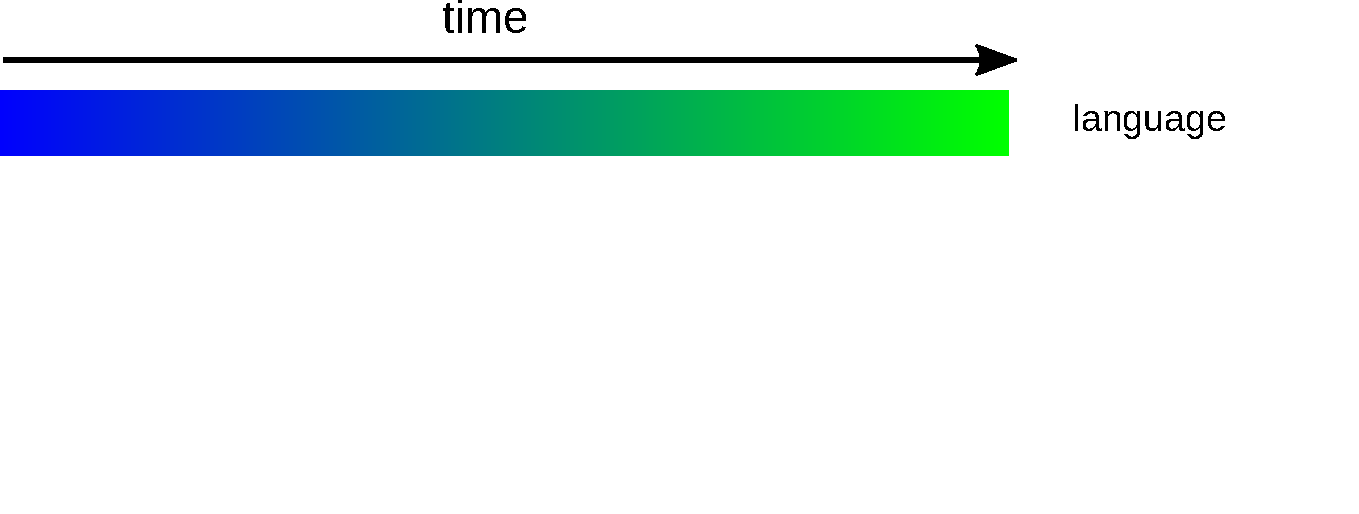
\includegraphics[width=\textwidth]{internalchange.pdf}\vfill ~
}


\frame{
\vspace*{1cm}
\frametitle{Contact-induced change }
  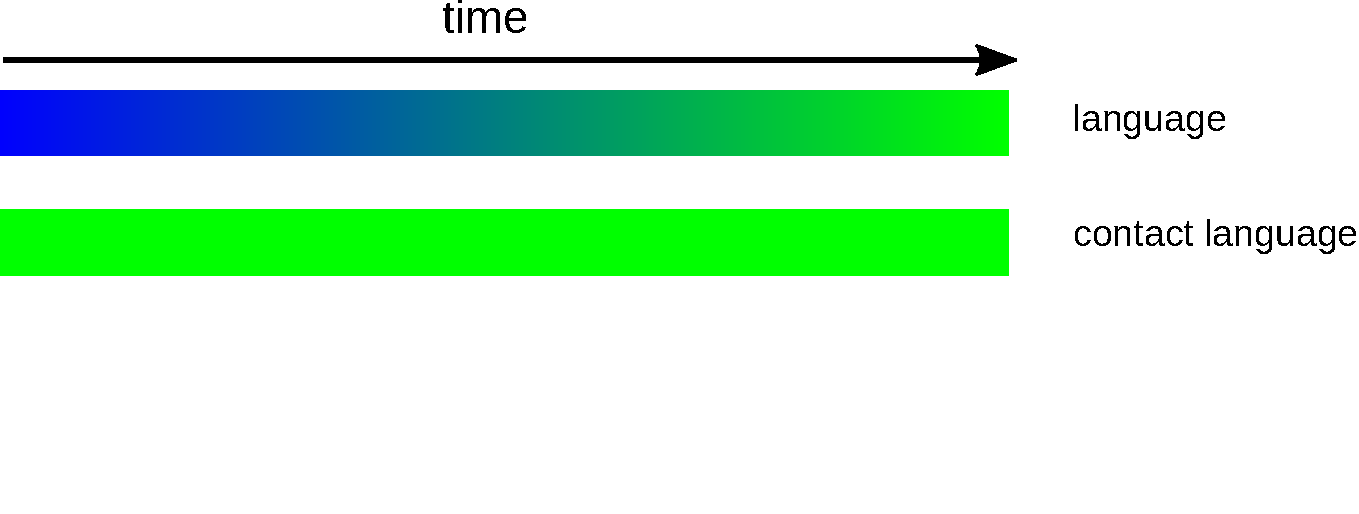
\includegraphics[width=\textwidth]{contactinducedchange.pdf}\vfill ~
}


\frame{
\vspace*{1cm}
\frametitle{Contact-induced non-change}
  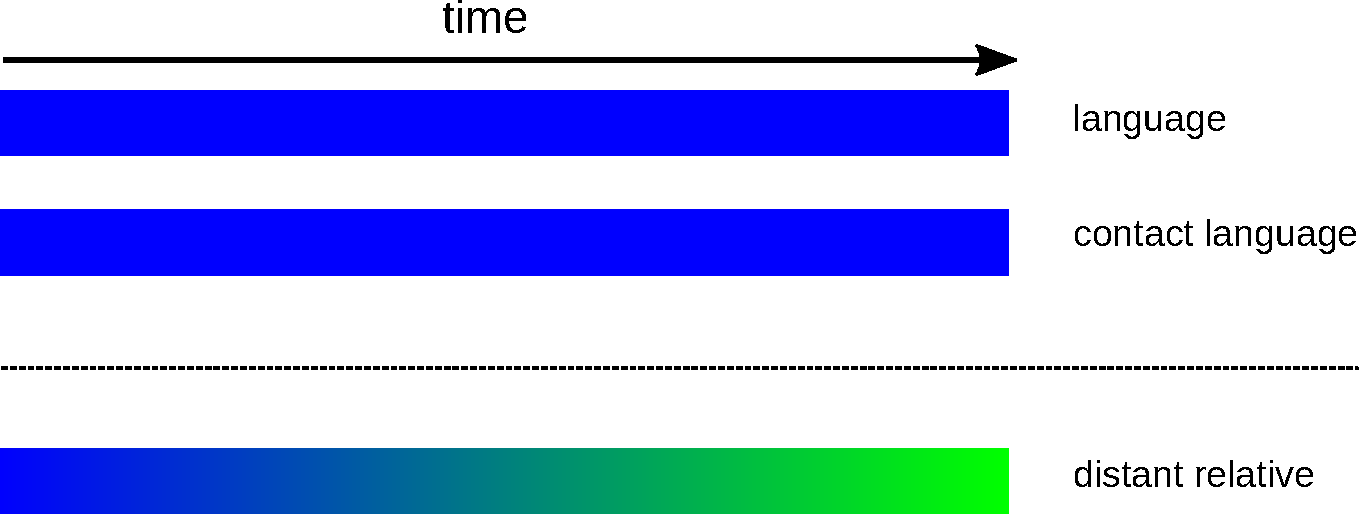
\includegraphics[width=\textwidth]{contactinducednonchange.pdf}\vfill ~
}


\frame{
\vspace*{1cm}
\frametitle{Contact-induced reversal}
  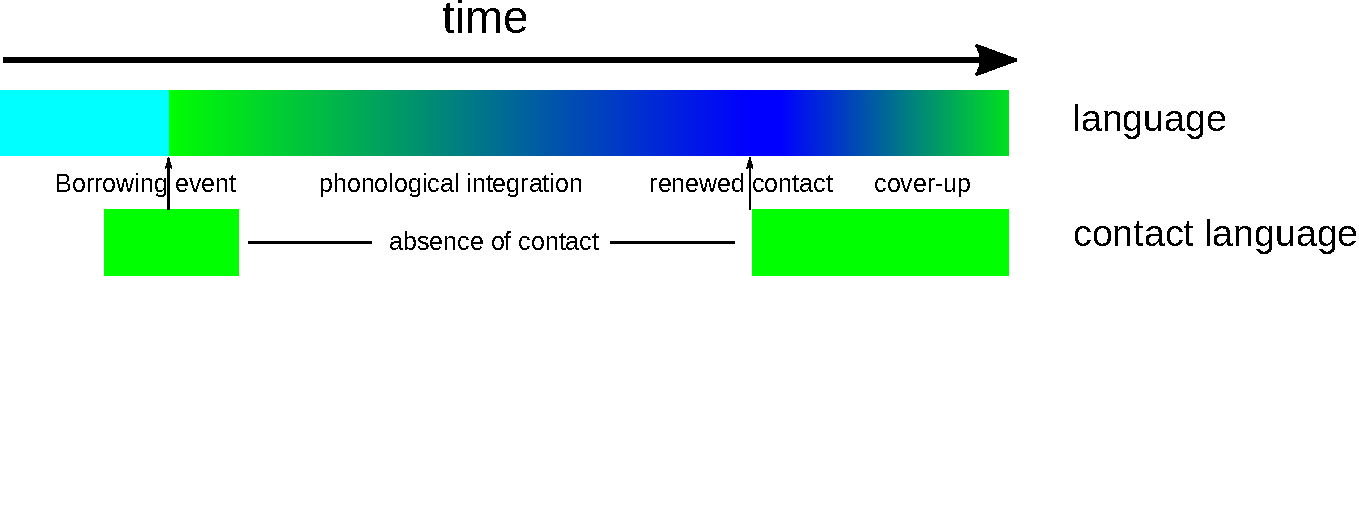
\includegraphics[width=\textwidth]{contactreversal.pdf}\vfill ~
}

\section{The setting}

\frame{
\frametitle{The setting}
  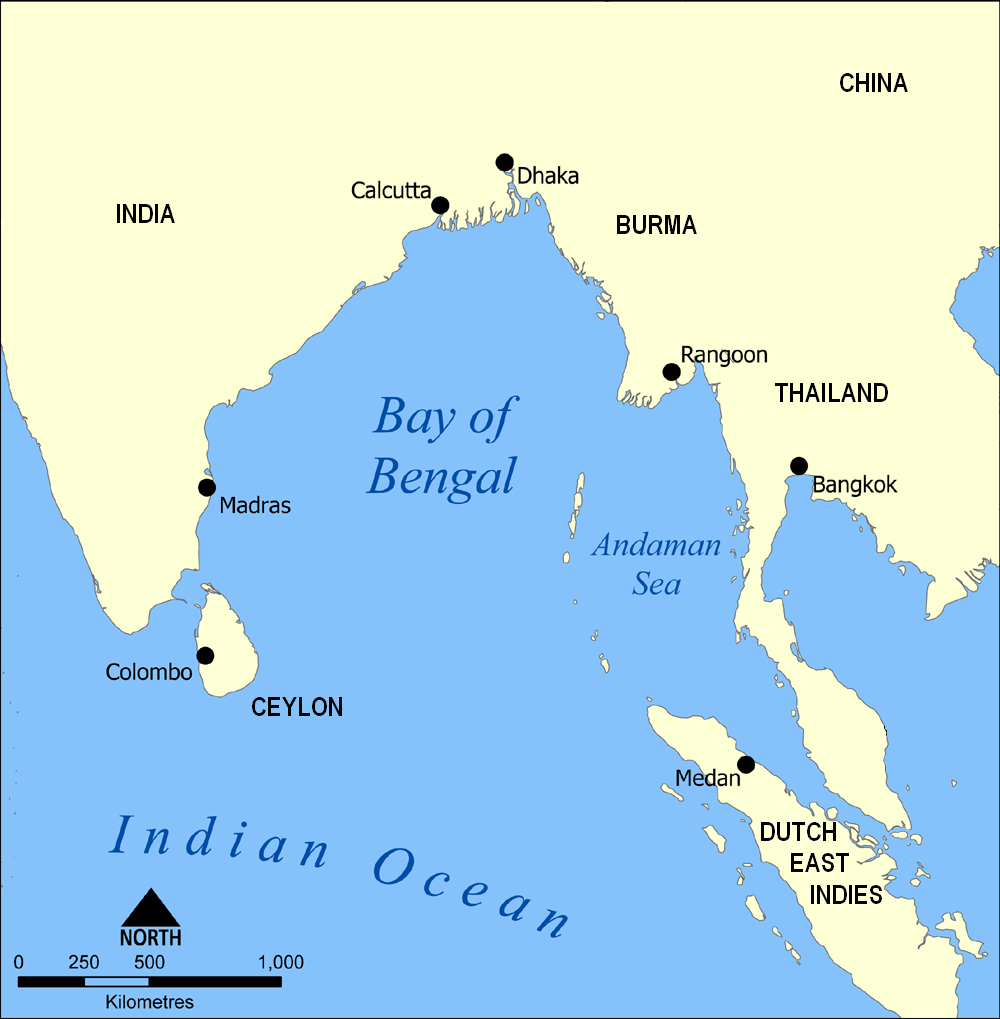
\includegraphics[height=.6\textheight]{BayofBengal.png}
  {\tiny \url{https://upload.wikimedia.org/wikipedia/commons/a/a0/Bay_of_Bengal_map_1800s.png}
    User:NormanEinstein made the original map, User:Ruhrfisch removed modern state borders, two cities, and changed three country names so it is suitable for 19th century articles., CC BY-SA 3.0 <http://creativecommons.org/licenses/by-sa/3.0/>, via Wikimedia Commons
}
}

\frame{
\frametitle{The setting}
 \begin{itemize}
    \item Monsoon Asia
    \item Either side of the Bay of Bengal
    \item In the West: South Asian Sprachbund \citep{Masica1976}
    \item In the East: the Malysian peninsula and archipelago
    \item long standing trade relations
    \item precolonial language contact
    \item loanwords from
    \begin{itemize}
      \item Hindi  \citep{Hamilton1919,Jones2007} % https://www.jstor.org/stable/41561311
      \item Tamil \citep{Hamilton1919,Jones2007,Hoogervorst2015}
      \item other Indian languages  \citep{Hamilton1919,Jones2007}
    \end{itemize}
  \end{itemize}
}



\section{Comparison}
\frame{
\frametitle{comparison}
\begin{tabular}{ll}
\toprule
Indian sprachbund & Malay world \\
\midrule
     two coronal places of articulation    &     one coronal place of articulation   \\
         ~~dental                            &                                         \\
         ~~retroflex                         &                                         \\
\tablevspace
     vowel length                          &     no distinctive vowel length         \\
\tablevspace
     geminate consonants                   &     no distinctive consonant length     \\
\tablevspace
     aspirated consonants                  &     no aspirated consonants             \\
\bottomrule
\end{tabular}
}


\section{Indian loanwords in Malay}
\frame{
\frametitle{Indian loanwords in Malay}
 \begin{itemize}
    \item     predictably lose their Indian features
    \item     phonological integration
    \begin{itemize}
    \item     \textit{kathā} $\to$ \textit{kata} `word'
      \begin{itemize}
        \item loss of aspiration, vowel length
      \end{itemize}
    \item     \textit{bhāṣā} $\to$ \textit{bahasa} `language'
      \begin{itemize}
        \item split of aspiration, vowel length, fronting of retroflex sibilant
      \end{itemize}
    \item     \textit{kaṭṭil} $\to$ \textit{katil} `bed'
      \begin{itemize}
        \item degemination, fronting of retroflex stop
      \end{itemize}
    \end{itemize}
    \item     \citet{Hamilton1919,Jones2007,Hoogervorst2015}
 \end{itemize}
}



\section{Sri Lanka Malay}
\frame{
\frametitle{Sri Lanka Malay}
 \begin{itemize}
    \item   language of the ethnic group of Malays in Sri Lanka
    \begin{itemize}
      \item 46,000 Malays in Sri Lanka (0.3\% of the population)
    \end{itemize}
    \item   brought between roughly 1650 and 1850
    \begin{itemize}
      \item colonial powers of the Dutch and the British
    \end{itemize}
    \item   contact languages Sinhala (IA) and Tamil (Dravidian)
    \item   important language change with phenomenal speed ensues
    \item \citet{Nordhoff2009,Nordhoff2012ed}
  \end{itemize}
}

\frame{
\frametitle{Language contact:\\ new features}
  \begin{itemize}
    \item       Case clitics
    \item       SOV word order
    \item       Postpositions
    \item       participles, infinitives
    \item       dental/retroflex distinction
    \item       vowel length/consonant lenght
      \begin{itemize}
      \item           depends on analysis, one is sufficient to account for the other
      \end{itemize}
    \item       prenasalized consonants
 \end{itemize}
}



\section{The SLM word}
\frame{
\frametitle{Metrical structure of the SLM word}
\begin{itemize}
  \item most words have two syllables
  \item the penultimate syllable typically either has a coda (CVC) or a long vowel (CVV)
  \item well-formed words
  \begin{itemize}
      \item CVV.CV
      \item CVC.CV
  \end{itemize}
  \item generalization
    \begin{itemize}
      \item CVX.CV
    \end{itemize}
   \item analysis: extrametrical final syllable with a bimoraic foot constraint
   \begin{itemize}
    \item C(V$_\mu$X$_\mu$).<CV>
    \item \citet{Nordhoff2009}
   \end{itemize}
 \end{itemize}
}







\section{regular sound change}
\frame{
\frametitle{regular sound change}
 \begin{itemize}
    \item     \textit{nasi} $\to$ \textit{naasi} `rice'
    \item     \textit{cuci} $\to$ \textit{cuuci} `wash'
    \item     \textit{sopi} $\to$ \textit{soopi} `liquor'
    \item     \textit{mati} $\to$ \textit{maat̪i} `to die'
    \item     \textit{derapa} $\to$ \textit{draapa} `how much'
    \item     \textit{bəsar} $\to$ \textit{bìssar}  `big'
 \end{itemize}
}



\section{exceptions}
\frame{
\frametitle{exceptions}
 \begin{itemize}
    \item   expected
    \begin{itemize}
      \item       \textit{kapal} $\to$ \textit{*kaapal} `ship'
      \item       \textit{topi} $\to$ \textit{*t̪oopi} `hat'
      \item       \textit{katil} $\to$ \textit{*kaat̪il} `bed'
    \end{itemize}
    \item   found
    \begin{itemize}
    \item       \textit{kapal} $\to$ \textit{kappal}
    \item       \textit{topi} $\to$ \textit{t̪oppi}
    \item       \textit{katil} $\to$ \textit{kaṭṭil}
    \end{itemize}
 \end{itemize}
}


\section{similar phonological environments}
\frame{
\frametitle{similar phonological environments}
 \begin{itemize}
    \item  \textit{topi/sopi}
    \item  \textit{drapa/kapal}
    \item  \textit{katil/mati}
    \item  phonological conditioning unlikely
    \item  lexically specified
    \begin{itemize}
    \item      reason:  cognates in contact languages
    \item Tamil \textit{toppi, kappal, kaṭṭil}
    \item Sinhala \textit{toppiya} `hat (sg)', \textit{toppi} `hat (pl)'
    \end{itemize}
    \item  \textbf{``phonological cover-up''}
 \end{itemize}
}


\section{Other types of cover-up}
\frame{
\frametitle{other types}
 \begin{itemize}
    \item The preceding examples have been chosen because they are easy to grasp
    \item Could be explained as a straight new act of borrowing
    \item unlikely for high frequency concepts like BOAT, HAT, and BED
    \begin{itemize}
      \item no evidence for lexical gaps or functional differentiation
    \end{itemize}
    \item other, more involved domains of cover-up to be discussed now:
    \begin{enumerate}
    \item  syllabification of ng
    \item  heterosyllabic NC clusters
    \item  re-fronting of voiced coronal stop
    \item unlengthening  of /u/
    \end{enumerate}
    \end{itemize}
    }

\frame{
\frametitle{Syllabification of ng}
\begin{itemize}
  \item Malay varieties can have syllable initial {\ng}
  \item So can Sri Lanka Malay
  \begin{itemize}
    \item      \textit{iŋat} $\to$ \textit{iiŋat̪} `to think'
   \end{itemize}
  \item based on this, we would expect \textit{siŋa} $\to$ \textit{*siiŋa} `lion'
  \item but we get
  \begin{itemize}
    \item      \textit{si.ŋa} $\to$ \textit{siŋ.ga}
  \end{itemize}
  \item explanation: Sinhala \textit{siŋ.ha.yaa} and Tamil \textit{ciŋ.gam} with a velar nasal coda in the first syllable
  \begin{itemize}
  \item Sanskrit \textit{siṃ.há}, Hindi \textit{siṅgh}\\
  ~~~~$\downarrow$
  \item resyllabification to \textit{si.ŋa} in Malay\\
  ~~~~$\downarrow$
  \item ``deresyllabfication''/cover-up in SLM to \textit{siŋ.ga}
  \end{itemize}
 \end{itemize}
}

\frame{
\frametitle{N ̬C clusters}
 \begin{itemize}
    \item   NC clusters with a voiced stop predicably have tautosyllabic rendering in SLM  (V.NCV)
    \begin{itemize}
    \item       \textit{gam.bar} $\to$ \textit{gaa.mbar} `picture'
  \end{itemize}
  \item exception
  \begin{itemize}
    \item       \textit{sam.bal} $\to$  \textit{*saa.mbal} `spicy dish'
    \item       \textit{sam.bal} $\to$ \textit{sam.bal}
  \end{itemize}
  \item explanation
  \begin{itemize}
    \item Tamil \textit{cam.bal}, Sinhala \textit{sam.bol} have heterosyllabic clusters
    \begin{itemize}
      \item NB: all Tamil clusters are heterosyllabic, but Sinhala has words with tautosyllabic clusters.
    \end{itemize}
  \end{itemize}
 \end{itemize}
}

\frame{
\frametitle{other types}
 \begin{itemize}
    \item  dental d
    \item      kalde $\to$ * kalde
    \item      kalde $\to$ kaldhe
    \item      kaLudhai
 \end{itemize}
}

\frame{
\frametitle{other types}
 \begin{itemize}
    \item   (guru)
    \item       guru $\to$ *guuru
    \item       guru $\to$ guru
 \end{itemize}
}

\section{metalinguistic awareness}
\frame{
\frametitle{metalinguistic awareness}
 \begin{itemize}
    \item  speakers are highly multilingual and are also able to identify cognates
    \item  buumi
    \item  Speakers
 \end{itemize}
}



\section{counter examples}
\frame{
\frametitle{counter examples}
 \begin{itemize}
    \item  rasa
    \item     kuda
 \end{itemize}
}


\section{Summary}
\frame{
\frametitle{Summary}
 \begin{itemize}
    \item  contact-induced reversal
    \item  speakers' metalinguistic awareness
    \item  "conscious" language change
    \item  phonological well-formedness helps
 \end{itemize}
}


\section{Outlook}
\frame{
\frametitle{Outlook}
 \begin{itemize}
    \item   What about other Sprachbund phenomena
    \item   Sinhala lost and recreated gemination several times during its history
    \item   German never created (and never lost) gemination
    \item   Is "inertia" in Sprachbunds also some kind of contact-induced non-change
    \item   crabs bucket
 \end{itemize}
}

\end{document}
